%\title{Overleaf Memo Template}

\documentclass[a4paper,11pt]{YuGroup}


\addbibresource{Exported_Items.bib} %change this to your .bib file These can be obtained by any citation manager. Export as biblatex file


\begin{document}
\maketitle



\section{Summary}
I have attempted to use some of the major functions in \LaTeX to write this document. In addition I tried to format things as close to rice's requirements as possible. \textbf{Always proofread your work.}  A full overview of \LaTeX is available on overleaf documentation also just google. There are lot of communities that use this. \par
 use \cite{noauthor_phase_nodate} to cite from the .bib file
\begin{figure}[H] %use [H] after the \being{figure} to keep figure where you want it
    \centering
    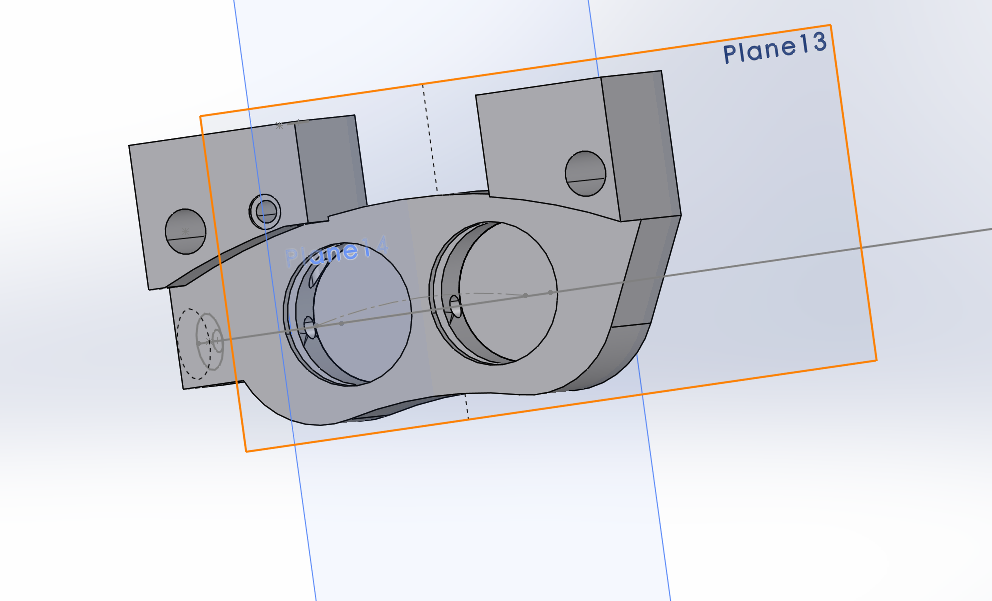
\includegraphics[scale=.75]{brake caliper.PNG}
    \caption{Im a caption}
    \label{fig:my_label}
\end{figure}
\section{Introduction and Background}

im a reference to \cref{fig:my_label} use me to reference figures ;lkadsflk;jasdf;lkajsd;lkjasddf;lkjasdd;
flkjasdjkjlkhjklhjklhlkjhkljhkljdf;lkjasdf;lkj \par %see this for paragraph stuff

latex makes inline equations easy
\begin{math}
    E = \frac{mc^2}{1}
\end{math}
dslakfjal;sdfl;asjdf;lkajsdf \par
also numbered equations
\begin{equation} %note the difference being equation and math
    e = v_{be} * I^{re}
\end{equation}
\section{Results and Discussion}

here is a table 
\begin{longtable}{lll}
\caption{Values used in equations 1 and 2}
\label{tab:my-table}\\
Parameter & Symbol & Value \\
\endhead
%
Voltage & V & 5V \\
Amperage & A & 1A
\end{longtable}

\subsection{Wow subsections}
\subsubsection{even further}


\section{Conclusions}
\appendix
\section{Appendix I}
use this for matlab

\lstinputlisting[style=matlab-editor]{FlatPlate.m}
 
\printbibliography % I make the reference section


\end{document}
